\subsection{plane conics and conic surfaces}

\subsubsection{the question of degeneracy}

A plane conic is a algebraic variety $\V(g)$ given by a quadratic form $g \in k[x_0,x_1,x_2]$. One might ask the question whether the conic is a union of two lines (in which case the conic is called \emph{degenerate}), or in algebraic terms, whether $g$ factors into two linear forms or whether it is irreducible.
Let's turn our attention the an easier question: When is a conic singular?

Assume that the characteristic of our base field $k$ is not 2, then the conic can be written, for appropriate coefficients $a,b,c,d,e,f \in k$ as:
\begin{equation}
g = ax_0^2 + bx_0x_1 + cx_1^2 + dx_0x_2 + ex_1x_2 + fx_2^2
\end{equation}
The singular points are given by the system of equations
\begin{equation}
\del_{x_0} g = \del_{x_1} g = \del_{x_2} g = 0
\end{equation}
which written out in matrix notation, amounts to
\begin{align}
\underset{=:M}{\underbrace{
\begin{pmatrix}
2a & b & e \\
b & 2c & d \\
e & d & 2f
\end{pmatrix}
}}
\begin{pmatrix}
x_0 \\ x_1 \\ x_2
\end{pmatrix}
= 0
\end{align}
We call the matrix $M$.
A singular point $[s_0:s_1:s_2] \in \proj^2_k$ would of course be a non-zero solution of above equation and as such can only exist precisely if the determinant of $M$ vanishes.
So far we have obtained

\begin{corollary}
Let $k$ be a field of characteristic not 2 and $g =  ax_0^2 + bx_0x_1 + cx_1^2 + dx_0x_2 + ex_1x_2 + fx_2^2
\in k[x_0,x_1,x_2]$ be a quadratic form. The conic $\V(g) \subset \proj^2_k$ is singular if and only if
\begin{equation}
\frac 12
\det
\begin{pmatrix}
2a & b & e \\
b & 2c & d \\
e & d & 2f
\end{pmatrix}
= 4acf + bde - ce^2 - ad^2 - b^2f = 0
\end{equation}
\end{corollary}

Incidentally this statement holds true for characteristic 2 as well, even though we need to approach the proof a little differently.
At this point I remind the reader that addition and subtraction are the same in characteristic 2, in the sense that negation operation is just the identity, which will simplify the calculations a little.
The corollary then translates to $g$ having a singular point if and only if $bde + ce^2 +ad^2 + b^2f = 0$.
The set of singular points is by definition the intersection of $V = \V(\del_{x_0}g,\del_{x_1}g,\del_{x_2}g)$ and $\V(g)$, so let's calculate the points in the first variety: Assuming that not all coefficients $b,f,e$ vanish, the only point on $V$ is $[e:d:b]$, as can be seen by Gaussian elimination where we distinguish the cases of $0,1$ or $2$ of the coefficients $b,d,e$ vanishing.
This point $[e:d:b]$ lies on $\V(g)$ iff $0 = g(e,d,b) = ae^2 + bde + cd^2 + dbe + ebd + fb^2 = bde + ae^2 + cd^2 + fb^2$ as desired.
If all of $b,d,e$ vanish, then $V$ is the whole space and every point of $\V(g)$ is singular ($\V(g) = \V((\sqrt{a}x_0 + \sqrt{c}x_1 + \sqrt{f}x_2)^2)$ being a doubled line) and also $bde + ce^2 + ad^2 + b^2f = 0$. We have proven:

\begin{corollary}
Let $k$ be a field of any characteristic and $g = ax_0^2 + bx_0x_1 + cx_1^2 + dx_0x_2 + ex_1x_2 + fx_2^2
 \in k[x_0,x_1,x_2]$ be a quadratic form. The conic $\V(g) \subset \proj^2_k$ is singular if and only if $4acf + bde - ce^2 - ad^2 - b^2f = 0$.
\end{corollary}


Returning to our initial question we want to establish the fact that the conic given by the quadratic form $g$ is irreducible if and only if it is non-singular.
For that assume reducibility, that is $g = h_1h_2$ for 1-forms $h_1$ and $h_2$.
We can apply the following lemma
\begin{lemma} \label{lemmaSingularIntersect}
Let $\V(I),\V(J)$ be two varieties. Then the union of $\V(IJ)$ is singular at their intersection $\V(I,J)$.
\end{lemma}
\begin{proof}
Let $f\in I, g\in J$, $P\in \V(I,J)$. We get $(fg)^{(1)}(P) = f(P)g^{(1)}(P) + g(P)f^{(1)}(P) = 0$, hence the tangent space at $P$ is the whole space.
\end{proof}
It says that the intersection of the two lines $\V(h_1)$ and $\V(h_2)$ (and we've seen that lines in $\proj^2_k$ do indeed intersect) is a singular point of our conic.

The converse can be seen as follows. Let $P=[p_0:p_1:p_2]$ be a singularity and $P'=[p'_0:p'_1:p'_2]$ is any other point on the conic (for instance any intersection point of $\V(g) \cap \V(x_i)$).
For $g$ to contain the line through $P$ and $P'$ means that $g(\lambda P + \mu P') = 0 \in k[\lambda,\mu]$.
Again, Euler's equality shows itself to be quite useful in the calculation
\begin{align}
0
= 2f(\lambda P')
=& \sum_{i=0}^2 \lambda p'_i \del_{x_i}g(\lambda P') 
+ \sum_{i=0}^2 \lambda p'_i \underset{=0}{\underbrace{\del_{x_i}g(\mu P)}}
\\
\overset{\del_{x_i}g\text{ is linear }}=& \sum_{i=0}^2 \lambda p'_i \del_{x_i} g(\lambda P'+\mu P) 
\\
=& 2g(\lambda P' + \mu P) - \sum_{i=0}^2 \mu p_i \del_{x_i}g(\lambda P' + \mu P)
\end{align}

Finally I claim that the last sum disappears due to the equality
\begin{equation}
\sum_{i=0}^2 p_i \del_{x_i}g = 0 \in k[x_0,x_1,x_2]
\end{equation}

The calculation is straight-forward:
\begin{align}
\sum_{i=0}^2 p_i \del_{x_i} g
=& \sum_{i=0}^2 p_i \sum_{j=0}^2 (\del_{x_j}\del_{x_i}g)x_j
\\
\overset{\text{lemma \ref{lemmaPartialDerivativesCommute}}}=& \sum_{j=0}^2 x_j \sum_{i=0}^2 (\del_{x_i}\del_{x_j}g)p_i = \sum_{j=0}^2 x_j \del_{x_j}g(P) = 0
\end{align}

Now that we have shown the sum to disappear, we obtain $0 = 2g(\lambda P' + \mu P)$ (in characteristic not 2), hence the conic contains a line.

For characteristic 2 I give a separate proof, as Euler's formula does not lead anywhere:
For $g$ to be singular at $P$ means that the following relations hold:
\begin{align}
bp_1 + dp_2 =& 0\\
bp_0 + ep_2 =& 0\\
dp_0 + ep_1 =& 0
\end{align}
With this we may write out $g(\lambda P + \mu P')$:
\begin{align}
a(\lambda p_0 + \mu p'_0)^2
+c(\lambda p_1 + \mu p'_1)^2
+f(\lambda p_2 + \mu p'_2)^2 \\
+b (\lambda p_0 + \mu p'_0)(\lambda p_1 + \mu p'_1)
+d (\lambda p_0 + \mu p'_0)(\lambda p_2 + \mu p'_2)
+e (\lambda p_1 + \mu p'_1)(\lambda p_2 + \mu p'_2)
\end{align}

Upon expanding we may collect the $\mu\lambda$ terms and see that they vanish after applying the previous three relations.
Furthermore the quadratic terms we have the equality (by means of the Frobenius homomorphism)
$a(\lambda p_0 + \mu p'_0)^2 = a\lambda^2p_0^2 + a \mu^2 {p'}_0^2$ etc.
It turns out, that after having done these transformations we get the equality $P(\lambda P + \mu P') = P(\lambda P) + P(\mu P') = 0$ as desired.
All in all we have shown:

\begin{theorem}
Let $k$ be a field and $\V(g) \subset \proj^2_k$ a conic given by a quadratic form $g = ax_0^2 + bx_0x_1 + cx_1^2 + dx_0x_2 + ex_1x_2 + fx_2^2$.
Then the following are equivalent:
\begin{enumerate}
\item The conic is degenerate.
\item The quadratic form $g$ factors into two linear forms, $g=h_1h_2$.
\item $\V(g)$ is a union of two lines.
\item $\V(g)$ is singular.
\item $4acf + bde - ce^2 - ad^2 - b^2f = 0$
\end{enumerate}
\end{theorem}


\begin{remark}
Otto Hesse has shown that over $k=\complex$ a curve $\V(g)$ decomposes into lines iff the Hessian curve $\V(\det(\del_{x_i}\del_{x_j}h))$ lies in $\V(g)$ (\cite[p.289]{brieskorn2012plane}), however we've seen that this result does not hold over arbitrary fields.
The equation of the Hessian curve in case of the conic considered in this section is precisely $2(4acf + bde - ce^2 - ad^2 - b^2f) = 0$.
\end{remark}


\subsubsection{the two rulings of a nonsingular quadric surface}


It is now time to profit from the previous meditations about singularities.
Let $Q \subset \proj^3_k$ be a non-singular quadric surface.
We will see that it does not make sense to count the lines on this surface, but let's find some first.
Surely $Q$ will not contain any plane, as this would mean (appealing to the Nullstellensatz) that $Q$ is the union of two planes.
Furthermore these planes intersect at least in a line, so by lemma \ref{lemmaSingularIntersect} the quadratic surface would be singular.
As a first step, choose a point $P \in Q$.
Because $Q$ does not contain planes, the tangent space intersects $Q$ in a conic curve.
This curve is singular at $P$ by lemma \ref{lemmaIntersectionWithTangent}, therefore it is the union of two lines $L_1,L_2$.

Each $L_i$ gives a family of lines as follows: For a point $P'$ on $L_i$, we may intersect again $Q$ with $T_{P'}Q$. Here too we obtain the union of two lines, one of which being $L_i$, the other line we call $L_i(P')$.
By this definition $L_1(P) = L_2$ and $L_2(P) = L_1$.
In fact, these are all the lines on $Q$, which is obvious from the following consideration.
Let $Z$ be any line on $Q$ which is neither $L_1$ nor $L_2$, then it intersects the plane $T_P(Q)$ in one point ($T_P(Q) \cap Z$ is the intersection of 3 hyperplanes).
This point lies precisely on one of the two $L_i$ (suppose that was not the case, then $Z \subset Q \implies Z = T_P(Z) \subset T_P(Q) \implies Z=L_1 \text{ or } Z=L_2$) so $Z = L_i(T_P(Q)\cap Z)$.
Conversely note, that we have chosen $P$ arbitrarily, so any point of $Q$ is the intersection of two lines $M_1,M_2$ on $Q$ and each of the two lines belong to the family $\{L_1(P')\}_{P'}$ or $\{L_2(P')\}_{P'}$.
It, however, cannot occur that both lines belong to the same family, say parametrised by $L_1$. In that case, $M_1,M_2,L_1$ would lie on the same tangent plane, but $Q$ intersects a tangent plane in just two lines!
We can conclude therefore:
\begin{proposition}
There are two families $\{ L_1(P') \}_{P'},\{ L_2(P') \}_{P'}$ of lines on $Q$ and each line on $Q$ belongs to one family. The lines in each family are disjoint and as set the union of any one family covers all of $Q$.
\end{proposition}

\begin{figure}
\center
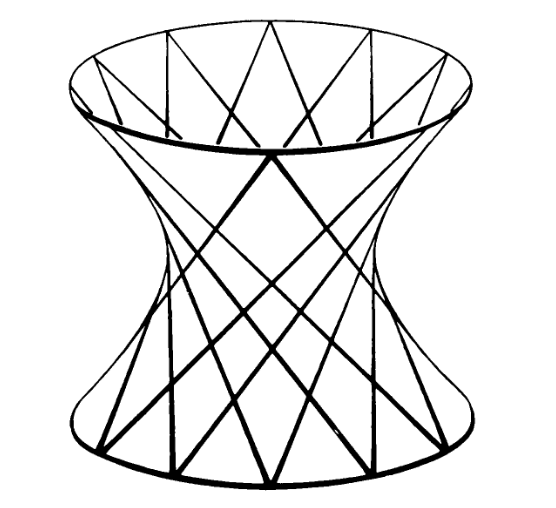
\includegraphics[width=.4\textwidth]{img/ruledsurface-hilbert.png}
\caption{An illustration of the rulings on the quadric surface `Anschauliche Geometrie' by Hilbert and Cohn-Vossen \cite[figure 17]{cohn1990geometry}}
\end{figure}

\begin{remark}
Over an algebraically closed field, a line has infinitely many points, so one cannot hope for the number of lines on a quadric to be finite.
\end{remark}

\begin{remark}
The reader, who is familiar with the Segre map $\sigma : \proj^1_k \times \proj^1_k \to \proj^3_k, ([x:y],[z:t]) \mapsto [xz:xt:yz:yt]$ (\cite[example 2.11]{harris1992algebraic}) may ask how the `rulings' on the non-singular quadric relates to the (so called) `ruled surface' which is the image of $\sigma$.
In fact we can give a Segre-like map for parametrisations $\phi$ of $L_1$ and $\psi$ of $L_2$.
Every point of $P' \in Q$ is then the some unique intersection $L_1(\phi([x:y])) \cap L_2(\psi([y:z]))$, giving a bijective map $Q \to \proj^1_k \times \proj^1_k, P' \mapsto ([x:y],[z:t])$.
\end{remark}


\begin{lemma} \label{lemmaThreeLines}
Three disjoint lines in $\proj^3_k$ lie on a quadric surface.
Such a quadric surface is necessarily irreducible.
\end{lemma}
\begin{proof}
Let's show irreducibility first.
If three disjoint lines lie on a quadric surface, then this surface cannot be the union of two planes, as two lines on a plane would intersect.
On the existence of the quadric surface:
We are given three disjoint lines with ideals $(h_1,h_2), (h_3,h_4), (h_5,h_6)$, the $h_i$ being linear forms, and want to find a quadratic form $q \in k[x_0,..x_3]$, such that $(h_1,h_2) \cap (h_3,h_4) \cap (h_5,h_6) \supset (q)$ (meaning that the union of the lines contains $\V(q)$).
It suffices to find linear forms $\lambda,\lambda',\mu,\mu',\nu,\nu'$ such that
$\lambda h_1 + \lambda' h_2 = \mu h_3 + \mu' h_4 = \nu h_5 + \nu' h_6 =: q$.
Solving for the linear forms means solving a homogeneous system of linear equations in $6*4= 24$ variables and $3\binom{4}{2} = 18$ equations, which ensures the existence of $q \neq 0$.
\end{proof}
